% !TeX root = ../presentation.tex

\section{Solid}

% TODO: Dreiecksbild auf meisten Folien klein in Ecke für Ref.

\begin{frame}{Solid \footnotesize\cite{mecklerWebLinkedData2023}}
    \begin{columns}
        \begin{column}{0.6\textwidth}
            \begin{itemize}
                % mögliche Implementierung des Data Space Konzeptes basiert auf Solid
                \item Data Space Konzept basierend auf\\
                    \emph{Solid} (ehem. Social Linked Data)
                    % TODO: Herkunft von Social Linked Data
                \item<2-> Ziel: offene, dezentralisierte Netzwerke für souveränen Datenaustausch
                \item<3-> Definition von Protokollen für Verwaltung und Austausch von Daten, Zugriffskontrolle und Identitätsmanagement
            \end{itemize}
        \end{column}
        
        \begin{column}{0.4\textwidth}
            \begin{figure}
                
\includegraphics[width=0.5\textwidth]{./assets/solid_logo.pdf}
                \caption{Solid-Logo~\cite{solidcommunitygroupSolidemblemsvg2019}}
                % TODO: Anw. <-> Daten // Lücke ID <-> Anw.
                % "identifiziert" --> "Identifizierung"
            \end{figure}
        \end{column}
    \end{columns}
\end{frame}


\begin{frame}{Solid II \footnotesize\cite{mecklerWebLinkedData2023}}
    \vspace{1em}
    \begin{figure}
        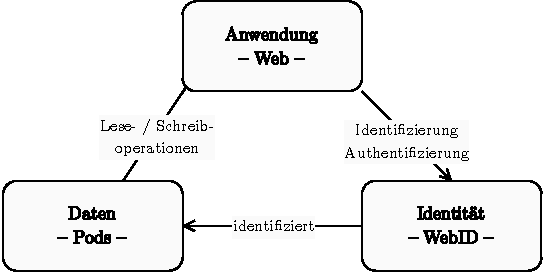
\includegraphics[height=5cm]{./assets/solid_triangle.drawio.pdf}
        \caption{Solid-Komponenten}
    \end{figure}
    % - Gliederung von Anwendungen in drei Teile
    %   - Anwendung als solches // Daten // Identität
    % - Identitätskomp.: verifiziert Identität eines Akteurs zur Auth. für Datenzugriff
    % - Daten und zugehörige Zugriffsregeln: dezentral in einen oder mehreren *Personal Online Data Stores* (Pods) gespeichert
    % - Anwendung verwendet ID, um korrekten Pod zu identifizieren und um sich für Datenzugriff zu auth.
    % - anschließend kann Anw. erforderliche Daten aus Pods lesen/schreiben
\end{frame}


\begin{frame}{Solid III \footnotesize\cite{mecklerWebLinkedData2023}}
    \begin{columns}
        \begin{column}{0.4\textwidth}
            \begin{itemize}
                \item Trennung und Standardisierung
                \item[$\Rightarrow$] Austauschbarkeit von Komponenten
                \item[$\Rightarrow$] Schritt"=für"=Schritt"=Einführung
                
                \item[$\Rightarrow$]<2-> geringe Einstiegsbarriere
                \item[$\Rightarrow$]<2-> hohe Zugänglichkeit
            \end{itemize}
        \end{column}
        
        \begin{column}{0.6\textwidth}
            \begin{figure}
                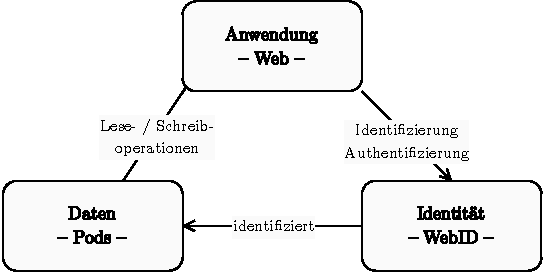
\includegraphics[width=\textwidth]{./assets/solid_triangle.drawio.pdf}
                % an Tafel malen
            \end{figure}
        \end{column}
    \end{columns}
\end{frame}


\subsection{Datenmanagement und Datenzugriff}

\begin{frame}{Datenstruktur}
    \begin{itemize}
        \item dezentrale Speicherung in \emph{Personal Online Data Stores} (Pods)~\cite{mecklerWebLinkedData2023,sambraSolidPlatformDecentralized2016}
        \item Standardisierung $\to$ Interoperabilität auf Daten"= statt Anwendungsebene
        % --> einfacher Wechsel von Anwendungen ohne aufwendige Datenmigration
        
        \item Binärdaten\only<1|handout:0>{?} \only<2->{mit Metadaten}
        % TODO: Durchstreichen
        
        \pause
        \pause
        \item lesbares Format \only<4->{$\to$ \emph{Resource Description Framework} (RDF) mit \emph{Vocabularies}~\cite{mecklerWebLinkedData2023,sambraSolidPlatformDecentralized2016}}
        % bspw. <Tim Berners-Lee> <is a> <person> (vgl. Bizer)
        % TODO: RDF-Erklärung höchstens kurz !!!
        
        \pause
        \pause
        \item Verknüpfung via \emph{Linked Data} $\to$ Struktur \& automatisierbare Semantik~\cite{bizerLinkedDataStory2009,mecklerWebLinkedData2023}

        \pause
        \item global eindeutige Identifikation via \emph{Uniform Resource Identifier} (URI)~\cite{sambraSolidPlatformDecentralized2016}
        \begin{itemize}
            \item \texttt{https://www.w3.org/People/Berners-Lee/card\#i}~\cite{bizerLinkedDataStory2009}
        \end{itemize}
        
        \pause
        \item Zugriffskontrolle auf jeder Hierarchie-Ebene mittels \emph{Access Control List} (ACL)
        
        \pause
        \item Mapping anderer Strukturen zu RDF~\cite{mecklerWebLinkedData2023,sambraSolidPlatformDecentralized2016}
    \end{itemize}
\end{frame}


% \begin{frame}{Datenstruktur II \footnotesize\cite{mecklerWebLinkedData2023,sambraSolidPlatformDecentralized2016}}
%     \begin{columns}
%         \begin{column}{0.6\textwidth}
%             \begin{itemize}
%                 \item (nicht-) RDF"=Dateien in \emph{LDP"=Container}
%                 \item wiederum RDF"=Graph $\to$ Verschachtelung möglich
%                 \item Zugriffskontrolle auf jeder Ebene mittels \emph{Access Control List} (ACL)
%                 \begin{itemize}
%                     \item \texttt{resource.acl} oder \texttt{.acl}
%                 \end{itemize}

%                 \item<2> unterschiedliche Rechte pro Akteur / Container
%                 \item[$\Rightarrow$]<2> feingranularer Datenschutz und Zugriffskontrolle
%             \end{itemize}
%         \end{column}

%         \begin{column}{0.4\textwidth}
%             \vspace{1em}
%             \begin{figure}
%                 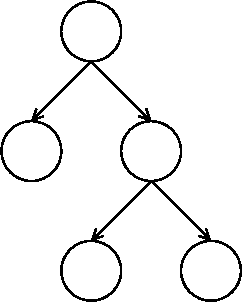
\includegraphics[height=4.5cm]{./assets/container_hierarchy.drawio.pdf}
%                 \caption{Hierarchie \cite[vgl.][]{sambraSolidPlatformDecentralized2016}}
%             \end{figure}
%         \end{column}
%     \end{columns}
% \end{frame}


\begin{frame}{Read- und Write-Protokoll \footnotesize\cite{mecklerWebLinkedData2023,sambraSolidPlatformDecentralized2016}}
    \begin{itemize}
        \item Anwendungen lesen und schreiben Daten direkt aus Pods
        \item Interoperabilität der Pods mit Anwendungen\\
            und wohldefiniertes, einfach implementierbares Protokoll
            % möglichst viel wiederverwenden, was bereits vorhanden ist
            % soll keine neue Komponenten sein --> aufbauend auf RESTful
        \item[$\Rightarrow$]<2-> RESTful"=Service, welche \emph{Linked Data Platform} (LDP) erfüllen
        \begin{itemize}
            % LDP: beschreibt Datenformat
            %   Einteilung in Ressourcen und Containern, Paging
            \item<2-> \texttt{HTTP GET}, \texttt{POST}, \texttt{PATCH}, \texttt{DELETE} etc.~\cite{sambraSolidPlatformDecentralized2016}
        \end{itemize}

        \item<3-> komplizierte Datenabfragen mittels SPARQL (optional)
    \end{itemize}
\end{frame}

% Fazit
% Datenmanagement betrachtet
% dezentrale Speicherung, Interoperabilität auf Daten- statt Anw.-Ebene
% Wie identifizieren wir Datenspeicher und Akteure für Datenzugriff? 

% \begin{frame}{Datenabfragen \footnotesize\cite{sambraSolidPlatformDecentralized2016}}
%     \begin{itemize}
%         \item nur einfache Abfragen mittels LDP"=Methoden möglich
%         \item komplizierte Datenabfragen mittels SPARQL (optional)
%         \item Delegation an Server $\Rightarrow$ Entwicklungsaufwand $\downarrow$

%         \pause
%         \item \emph{Local Queries}: innerhalb \emph{eines} Pods
%         \item \emph{Link Following Queries}: über mehrere Pods hinweg
%         \begin{itemize}
%             \item via Link"=Following
%             \item tatsächliche Verteilung muss nicht bekannt sein
%         \end{itemize}
%     \end{itemize}
% \end{frame}


\subsection{Identität und Authentifizierung}

\begin{frame}{Authentifizierung \footnotesize\cite{sambraSolidPlatformDecentralized2016}}
    \begin{itemize}
        \item Vertrauen, Datensouveränität und Datenschutz $\to$ Authentifizierung
        \item Dezentralisierung benötigt globalen \emph{Identity Space}
        
        \item<2-> passend zu RDF"=basierten Daten
        \item<2-> Ermittlung der Identität und Profildaten
        \item<2-> Ermittlung relevanter Links zum Pod und zu Anwendungsdaten
        
        \item[$\Rightarrow$]<3-> aktuell: \emph{WebID} (austauschbar)
        \item[$\Rightarrow$]<3-> globales Identitätsmanagement basierend auf System dezentralisierter \emph{Identity Provider}
    \end{itemize}
\end{frame}


\begin{frame}{Identität}
    \begin{columns}
        \begin{column}{0.55\textwidth}
            \begin{itemize}
                \item Akteure besitzen WebID"=URI~\cite{sambraSolidPlatformDecentralized2016}
                
                \item Referenz auf \emph{WebID Profile Document}~\cite{sambraSolidPlatformDecentralized2016,solidcommunitygroupSolidemblemsvg2019}
                
                \begin{itemize}
                    \item<2-> Referenz auf Pod und Anwendungsdaten~\cite{solidcommunitygroupSolidWebIDProfile2024}
                    \item<2-> Referenz auf weitere Profildaten~\cite{solidcommunitygroupSolidWebIDProfile2024}
                    % Webseite im RDF"=Format, global eindeutige URI~\cite{sambraSolidPlatformDecentralized2016}
                \end{itemize}
                
                \item<3-> Speicherung bei Identity Provider\\
                    (meist Pod Provider)~\cite{sambraSolidPlatformDecentralized2016}
                \item[$\Rightarrow$]<3-> Kontrolle über eigene Identität bei Nutzenden~\cite{sambraSolidPlatformDecentralized2016}
            \end{itemize}
        \end{column}

        \begin{column}{0.45\textwidth}
            \only<2->{
                \begin{figure}
                    \centering
                    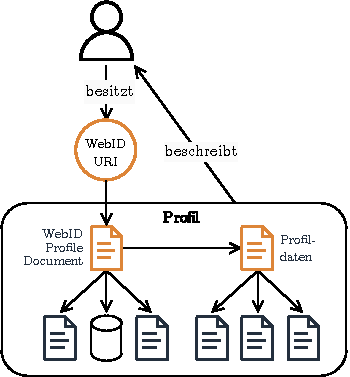
\includegraphics[height=5.5cm]{./assets/profile.drawio.pdf}
                    \caption{Solid Profil~\cite[vgl.][]{sambraSolidPlatformDecentralized2016,solidcommunitygroupSolidWebIDProfile2024}}
                    % TODO: WebID URI Rand kleiner
                \end{figure}
            }
        \end{column}
    \end{columns}
\end{frame}


\begin{frame}{Web of Trust \footnotesize\cite{sambraSolidPlatformDecentralized2016}}
    \begin{columns}
        \begin{column}{0.6\textwidth}
            \begin{itemize}
                \item Verknüpfung von Identitäten über mehrere Seiten\\
                $\Rightarrow$ \emph{Web of Trust}
                % hilfreich, da man nicht alle Akteure in einem DS / DE kennen kann
                
                \item[$\Rightarrow$]<2-> ad-hoc Auth.-Entscheidungen basierend auf Profileigenschaften
                % bspw. Beziehungen zu anderen Akteuren, Arbeitsstelle, Teil einer Gruppe etc. etc.
                % transitives Vertrauen
                
                \item[$\Rightarrow$]<3-> Wem kann ich vertrauen?\\ Kann ich den geteilten Daten vertrauen?
                
                \item[$\Rightarrow$]<4-> Adressierung eines Kern"=Hindernisses
            \end{itemize}
            % aber wenn ein Akteur kompromittiert, dann SCHLECHT
        \end{column}
        
        \begin{column}{0.4\textwidth}
            \vspace{1em}
            \begin{figure}
                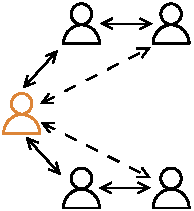
\includegraphics[height=4cm]{./assets/web_of_trust.drawio.pdf}
                \caption{Web of Trust}
            \end{figure}
        \end{column}
    \end{columns}
\end{frame}


\subsection{Erweiterung: Wertschöpfungsketten}

\begin{frame}{Erweiterung: Wertschöpfungsketten \footnotesize\cite{bothSolidBasedB2BData2025}}
    \begin{itemize}
        \item automatisierte Datenübertragung essenziell für Partner:in in Wertschöpfungsketten
        \item weitere Anforderungen
        \begin{itemize}
            \item garantierte, nachvollziehbare Einhaltung rechtlicher Rahmenbedingungen
            \item Constraints für Data Sharing
        \end{itemize}
    \end{itemize}

    \begin{figure}
        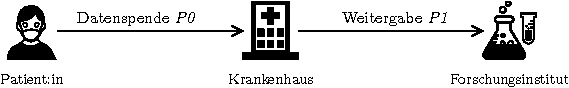
\includegraphics[width=\textwidth]{./assets/example_horizontal.drawio.pdf}
        \caption{Beispiel: Datenspende}
    \end{figure}
\end{frame}


\begin{frame}{Erweiterung: Wertschöpfungsketten II \footnotesize\cite{bothSolidBasedB2BData2025}}
    \addtocounter{figure}{-1}
    \begin{figure}
        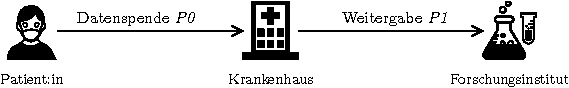
\includegraphics[width=\textwidth]{./assets/example_horizontal.drawio.pdf}
        \caption{Beispiel: Datenspende}
    \end{figure}
    
    \vspace{-1em}

    \begin{itemize}
        \item Einführung zusätzlicher Metadaten
        \begin{itemize}
            \item \emph{Data Processing Purpose} $P$ % Weitergabe muss sich trotzdem an ursprüngl. Zweck halte
            \item Verstecken der Datenquelle, Angabe über Weitergabe
        \end{itemize}

        \item<2-> weitere Validierung notwendig
        % weiterer Schritt in Richtung E2E-B2B-Wertschöpfungsketten
        % Möglichkeit und Notwendigkeit zur Erweiterung von Solid
    \end{itemize}

    % TODO: Stichpunkte zum Erzählen
\end{frame}
